\clearpage
%//==============================--@--==============================//%
%\vspace{-1em}
\subsection{P1 | Distribuição de probabilidades de equilíbrio dos estados do Monopólio simplificado.}
\label{subsec:P1}

%//==============================--A--==============================//%
%\vspace{-0.5em}
\subsubsection{a) Estados percorridos num \textit{run} e valores simulados para o resultado do lançamento da moeda nas sucessivas jogadas desse \textit{run}.}
\label{subsubsec:P1a}

\vspace{-1em}
\begin{figure}[H]
    \centering
    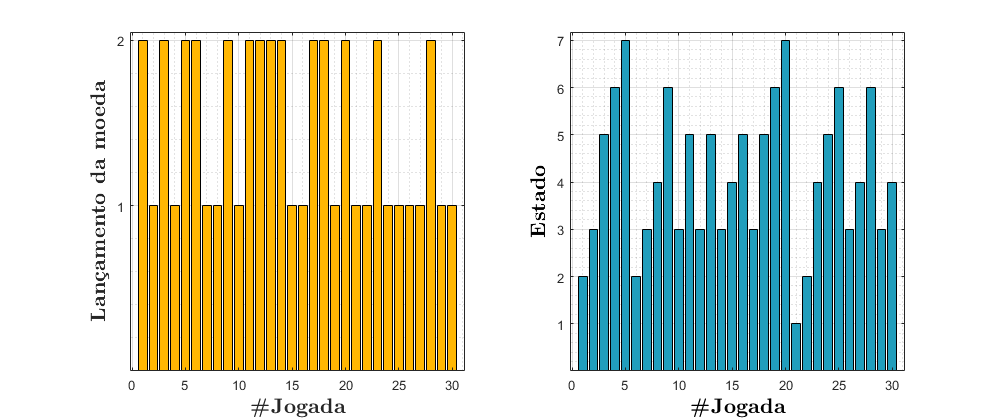
\includegraphics[width = 1\linewidth]{img/P1/P1a.png}
    \caption{Resultado do lançamento da moeda e estados percorridos numa \textit{run} com 30 jogadas\protect\footnotemark[2].}
    \label{fig:P1a}
\end{figure}
\noindent\textbf{\textit{$\rightarrow$ Observações}}

\begin{itemize}
    \item[$\blacktriangle$] O reduzido valor de iterações (jogadas) é escolhido para uma fácil visualização dos gráficos, já que, como veremos em seguida, este valor mostra-se insuficiente para garantir um regime estocástico estacionário.
    \item[$\blacktriangle$] De notar a elevada incidência no estado 3  e 5, resultado congruente com o vetor de equilíbrio (\textit{steady-state vector}) da cadeia em questão (vide \hyperref[subsec:intro]{secção introdutória})
\end{itemize}

%//==============================--A--==============================//%
\footnotetext[2]{Vide \hyperref[subsubsec:P2iii]{secção P2 iii)}.}
%//==============================--A--==============================//%
%//==============================--B--==============================//%
%\vspace{-0.5em}
\subsubsection{b) Frequências relativas dos diferentes estados (muitas jogadas), descartando um transitório inicial.}
\label{subsubsec:P1b}

\vspace{-1em}
\begin{figure}[H]
    \centering
    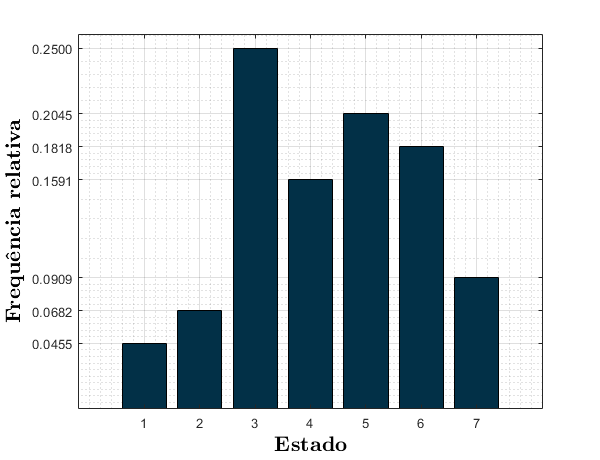
\includegraphics[width = 0.55\linewidth]{img/P1/P1b.png}
    \caption{Frequências relativas para uma simulação de 1000000 \textit{runs} cada uma com 1000 jogadas, de onde 20 são descartadas.}
    \label{fig:P1b}
\end{figure}

\noindent\textbf{\textit{$\rightarrow$ Observações}}
\begin{itemize}
    \item[$\blacktriangle$] Os \textit{steady-state values} simulados de cada estado aproximam-se rigorosamente dos valores teóricos expectáveis (\hyperref[subsec:intro]{secção introdutória}).
    \item[$\blacktriangle$] O valor de \textit{burn-in} (\textit{Ndiscard}) estipulado é o que garante a melhor eliminação do \textit{bias} inicial imposta pela influência da casa de partida ($x_0$).
    \item[$\blacktriangle$] A distribuição das probabilidades estacionárias por estado são intuitivamente explicadas pelo diagrama da cadeia: Sucintamente, $x_1$ é o estado menos provável, a transição (fora a eventual transição inicial do estado $x_0$) só é possível através de uma lançamento com resultado coroa do estado 7. $x_3$ é o estado mais provável, a transição é possível através do estado $x_1$ (coroa), $x_2$ (cara), $x_5$ (coroa) e $x_6$ (cara).   
\end{itemize}


%//==============================--C--==============================//%
%\vspace{-0.5em}
\subsubsection{c) Renda média em regime estocástico estacionário.}
\label{subsubsec:P1c}

Trivialmente se obtêm os valores de renda média efetuando o produto das entradas dos vetores zfreq e Aluguer (nomenclatura conforme o Guia Laboratorial): 
$$ \text{Renda média} = \left[\text{zfreq}(i) \cdot \text{Aluguer}(i)\right]\text{,}\  i = 1, \dots, 7 $$

\vspace{-1em}
\begin{figure}[H]
    \centering
    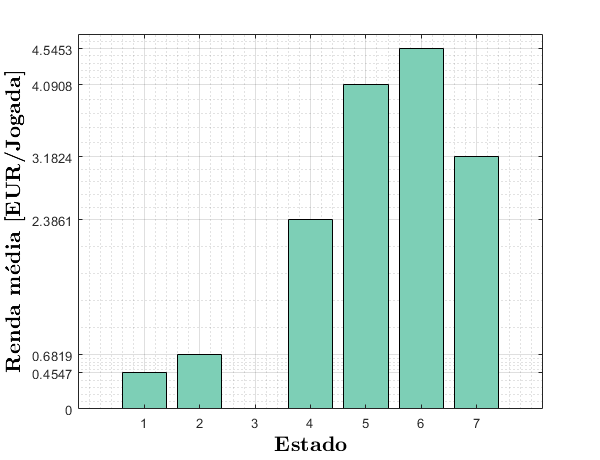
\includegraphics[width = 0.55\linewidth]{img/P1/P1c.png}
    \caption{Renda média para uma simulação de 1000000 \textit{runs} cada uma com 1000 jogadas, de onde 20 são descartadas.}
    \label{fig:P1c}
\end{figure}

\noindent\textbf{\textit{$\rightarrow$ Observações}}
\begin{itemize}
    \item[$\blacktriangle$] O estado 3 possui renda média nula, já que o pagamento é inexistente na prisão (como veremos na \hyperref[subsec:P4]{secção P4} o pagamento poderá equacionar em tempo).
    \item[$\blacktriangle$] A renda é tanto maior quanto maior for a frequência relativa e o preço de aluguer do respetivo estado.
\end{itemize}

%//==============================--@--==============================//%
